\documentclass{article}

% Language setting
\usepackage[english]{babel}
\usepackage{listings}
\usepackage{minted}
% Remove this draft watermark for the final version
% \usepackage{draftwatermark}

% Set page size and margins
% Replace `letterpaper' with `a4paper' for UK/EU standard size
\usepackage[letterpaper,top=2cm,bottom=2cm,left=3cm,right=3cm,marginparwidth=1.75cm]{geometry}

% Useful packages
\usepackage{amsmath}
\usepackage{comment}
\usepackage{graphicx}
\usepackage{IEEEtrantools}
\usepackage[hyphens]{url}
\usepackage[colorlinks=true, allcolors=blue]{hyperref}

\title{The Aptos Blockchain: Safe, Scalable, and Upgradeable Web3 Infrastructure}
\author{}
\date{\today\\v1.0}

\begin{document}
\maketitle

\begin{abstract}
The rise of blockchains as a new Internet infrastructure has led to developers deploying tens of thousands of decentralized applications at rapidly growing rates. Unfortunately, blockchain usage is not yet ubiquitous due to frequent outages, high costs, low throughput limits, and numerous security concerns. To enable mass adoption in the web3 era, blockchain infrastructure needs to follow the path of cloud infrastructure as a trusted, scalable, cost-efficient, and continually improving platform for building widely-used applications. 
 
We present the \emph{Aptos blockchain}, designed with scalability, safety, reliability, and upgradeability as key principles, to address these challenges. The Aptos blockchain has been developed over the past three years by over 350+ developers across the globe \cite{aptos_core_github}. It offers new and novel innovations in consensus, smart contract design, system security, performance, and decentralization. The combination of these technologies will provide a fundamental building block to bring web3 to the masses:\footnote{Legal Disclaimer: This white paper and its contents are not an offer to sell, or the solicitation of an offer to buy, any tokens. We are publishing this white paper solely to receive feedback and comments from the public. Nothing in this document should be read or interpreted as a guarantee or promise of how the Aptos blockchain or its tokens (if any) will develop, be utilized, or accrue value. Aptos only outlines its current plans, which could change at its discretion, and the success of which will depend on many factors outside of its control. Such future statements necessarily involve known and unknown risks, which may cause actual performance and results in future periods to differ materially from what we have described or implied in this white paper. Aptos undertakes no obligation to update its plans. There can be no assurance that any statements in the white paper will prove to be accurate, as actual results and future events could differ materially. Please do not place undue reliance on future statements.}
 
 \begin{itemize}
  \item First, the Aptos blockchain natively integrates and internally uses the \emph{Move language} for fast and secure transaction execution \cite{move_github}. The \emph{Move prover}, a formal verifier for smart contracts written in the Move language, provides additional safeguards for contract invariants and behavior. This focus on security allows developers to better protect their software from malicious entities. 
  \item Second, the Aptos data model enables flexible key management and hybrid custodial options. This, alongside transaction transparency prior to signing and practical light client protocols, provides a safer and more trustworthy user experience. 
  \item Third, to achieve high throughput and low latency, the Aptos blockchain leverages a pipelined and modular approach for the key stages of transaction processing. Specifically, transaction dissemination, block metadata ordering, parallel transaction execution, batch storage, and ledger certification all operate concurrently. This approach fully leverages all available physical resources, improves hardware efficiency, and enables highly parallel execution. 
  \item Fourth, unlike other parallel execution engines that break transaction atomicity by requiring upfront knowledge of the data to be read and written, the Aptos blockchain does not put such limitations on developers. It can efficiently support atomicity with arbitrarily complex transactions, enabling higher throughput and lower latency for real-world applications and simplifying development.
  \item Fifth, the Aptos modular architecture design supports client flexibility and optimizes for frequent and instant upgrades. Moreover, to rapidly deploy new technology innovations and support new web3 use cases, the Aptos blockchain provides embedded on-chain change management protocols. 
  \item Finally, the Aptos blockchain is experimenting with future initiatives to scale beyond individual validator performance: its modular design and parallel execution engine support internal sharding of a validator and homogeneous state sharding provides the potential for horizontal throughput scalability without adding additional complexity for node operators.
\end{itemize}

\end{abstract}

\section{Introduction}

In the web2 version of the Internet, services such as messaging, social media, finance, gaming, shopping, and audio/video streaming, are provided by centralized companies that control direct access to user data (e.g., Google, Amazon, Apple, and Meta). These companies develop infrastructure using application-specific software optimized for targeted use cases and leverage cloud infrastructures to deploy these applications to users. Cloud infrastructure provides access to virtualized and/or physical infrastructure services, such as rented virtual machines (VMs) and bare metal hardware operating inside data centers worldwide (e.g., AWS, Azure, and Google Cloud). As a result, building web2 Internet services that can scale to billions of users has never been easier than it is today. However, web2 requires that users place explicit trust in centralized entities, a requirement that has become increasingly concerning to society.

To combat this concern, a new Internet age has begun: web3. In the web3 version of the Internet, \emph{blockchains} have emerged to provide decentralized, immutable ledgers that enable users to interact with one another securely and reliably, all without requiring trust in controlling intermediaries or centralized entities. Similar to how web2 Internet services and applications rely on cloud infrastructure as building blocks, decentralized applications can use blockchains as a decentralized infrastructure layer to reach billions of users across the world.

However, despite the existence of many blockchains today, widespread adoption of web3 has not yet taken place~\cite{a16_state}. While technology continues to advance the industry, existing blockchains are  unreliable, impose high transaction fees for users, have low throughput limitations, suffer regular asset losses due to security issues, and cannot support real-time responsiveness. In comparison to how cloud infrastructure has enabled web2 services to reach billions, blockchains have not yet enabled web3 applications to do the same.

\section{The Aptos vision}

The Aptos vision is to deliver a blockchain that can bring mainstream adoption to web3 and empower an ecosystem of decentralized applications to solve real-world user problems. Our mission is to advance the state-of-the-art in blockchain reliability, safety, and performance by providing a flexible and modular blockchain architecture. This architecture should support frequent upgrades, fast adoption of the latest technology advancements, and first-class support for new and emerging use cases.

We envision a decentralized, secure, and scalable network governed and operated by the community that uses it. When infrastructure demands grow across the world, the computational resources of the blockchain scale up horizontally and vertically to meet those needs. As new use cases and technological advances arise, the network should frequently and seamlessly upgrade without interrupting users. Infrastructure concerns should fade into the background. Developers and users will have access to many different options for key recovery, data modeling, smart contract standards, resource usage trade-offs, privacy, and composability. Users know that their assets are secure, always available, and can be accessed with near at-cost fees.  Anyone can safely, easily, and immutably transact with untrusted parties worldwide. Blockchains are as ubiquitous as cloud infrastructure.

To achieve this vision, significant technological advances must be made. Our experiences building, developing, advancing, and deploying the Diem blockchain (the predecessor of the Aptos blockchain) over the past three years have proven that a network can continually upgrade its protocols without disrupting its clients \cite{diem_blockchain}. The Diem mainnet was deployed to more than a dozen node operators with multiple wallet providers in early 2020. Over the following year, our team issued two major upgrades that changed the consensus protocol and the core framework. Both upgrades completed without downtime for users. With the Aptos blockchain, we have made a series of radical improvements to the technology stack while also incorporating safe, transparent, and frequent upgrades as a core feature, as inspired by the Diem blockchain. In particular, we highlight novel methods of transaction processing (as described in Section \ref{sec:pipelining_batching}) and new approaches to decentralization and network governance.

As the Aptos blockchain continues to improve and grow, we will issue refreshed versions of this white paper with the latest iteration of our protocols and design choices. In the rest of this document, we describe the current state of the Aptos blockchain as well as future plans.

\begin{figure}
\centering
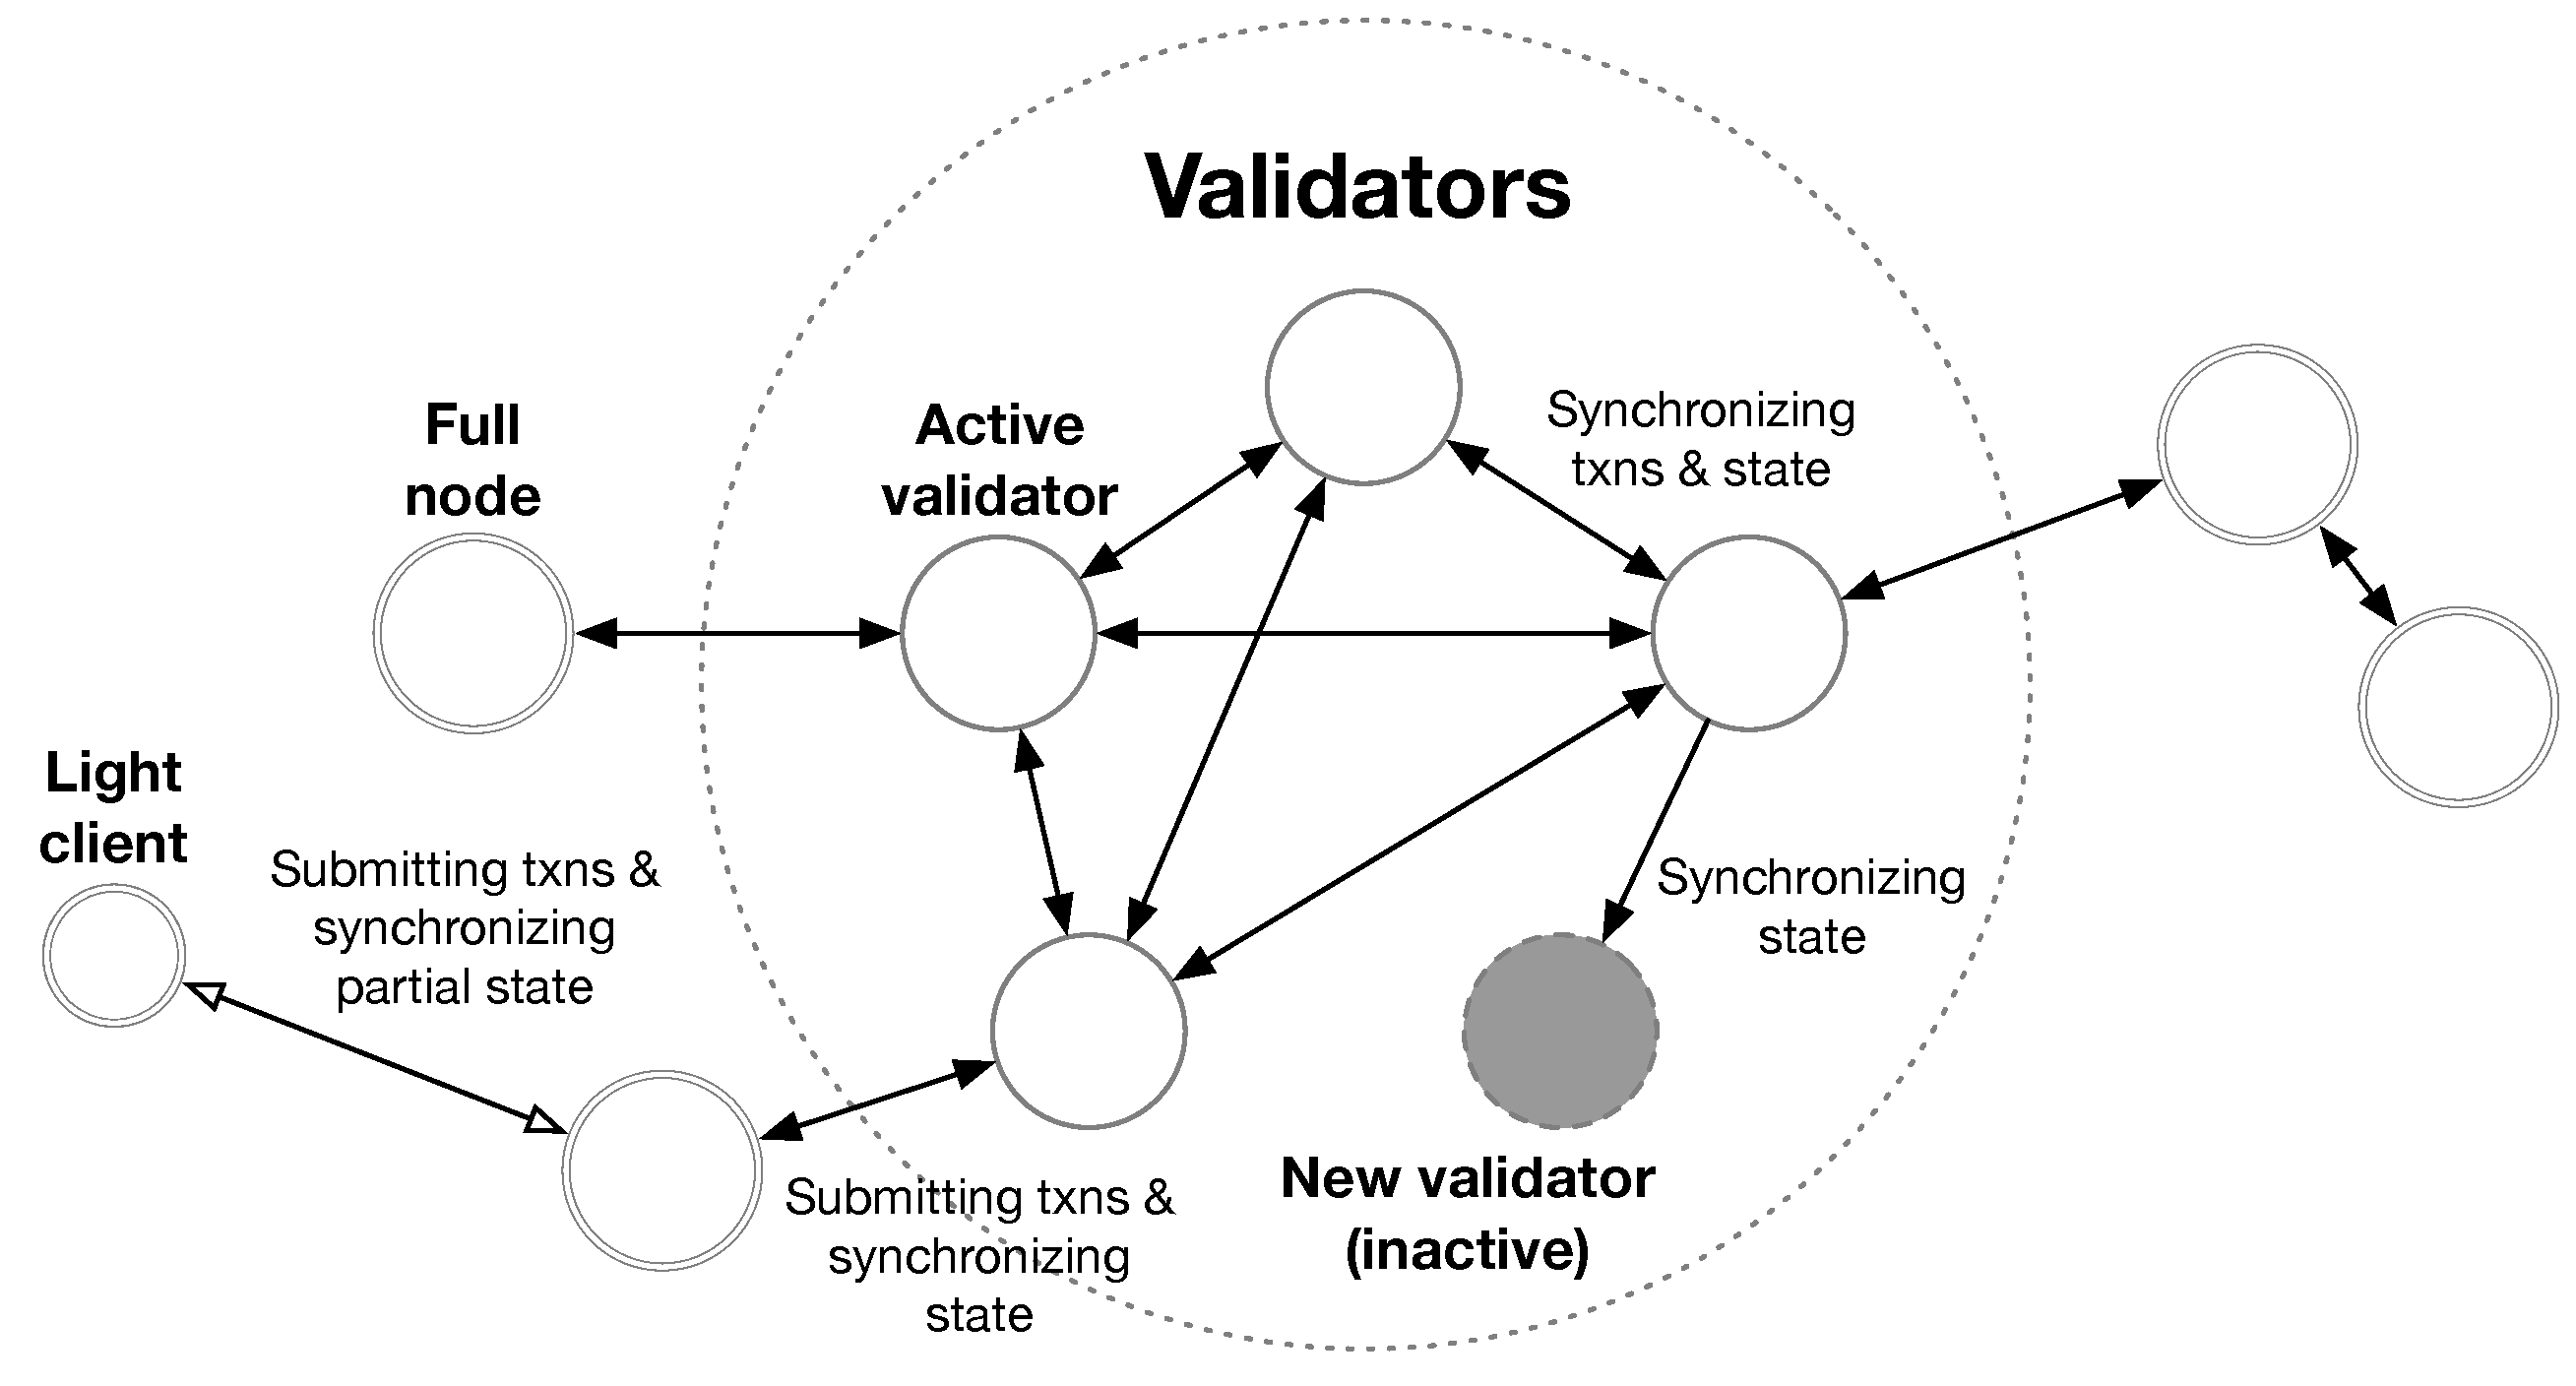
\includegraphics[width=0.9\textwidth]{validators.eps}
\caption{\label{fig:aptos_ecosystem}Components of the Aptos ecosystem.}
\end{figure}

\section{Overview}

The Aptos blockchain, as shown in Figure \ref{fig:aptos_ecosystem}, is comprised of a set of \emph{validators} that jointly receive and process transactions from users using a byzantine fault-tolerant (\emph{BFT}), proof-of-stake consensus mechanism. Token holders lock up, or \emph{stake}, tokens in their selected validators. Each validator's consensus voting weight is proportionate to the amount staked into it. A validator can be \emph{active} and participate in consensus. Likewise, a validator may also be \emph{inactive} if it does not have enough stake to participate, rotates out of the validator set, elects to be offline as it synchronizes blockchain state, or is deemed not participating by the consensus protocol due to poor historical performance.

\emph{Clients} are any part of the system that need to submit transactions or query the state and history of the blockchain. Clients can choose to download and verify validator signed proofs of queried data.
\emph{Full nodes} are clients that replicate the transaction and blockchain state from the validators or from other full nodes in the network. They may elect to prune transaction history and blockchain state as desired to reclaim storage.
\emph{Light clients} only maintain the current set of validators and can query partial blockchain state securely, typically from full nodes. Wallets are a common example of a light client.

To meet the needs of safe, fast, reliable, and upgradeable web3 infrastructure for widespread adoption, the Aptos blockchain is built on the following core design principles:

\begin{itemize}
\item Fast and secure execution along with simple auditability and mechanical analyzability via a new smart contract programming language, Move \cite{move}. Move originated with the predecessor to the Aptos blockchain and continues to progress with the evolution of this project.
\item Extremely high throughput and low latency through a batched, pipelined, and parallelized approach to transaction processing.
\item Novel parallel transaction processing that efficiently supports atomicity with arbitrarily complex transactions through Block-STM, unlike existing parallel execution engines that require upfront knowledge of data locations to be read and written.
\item Optimizations for performance and decentralization via rapid, stake-weight validator set rotation and reputation tracking.
\item Upgradeability and configurability as first-class design principles to embrace new use cases and the latest technology.
\item Modular designs that enable rigorous component level testing along with appropriate threat modeling and seamless deployment, all ensuring highly secure and reliable operations.
\item Horizontal throughput scalability while preserving decentralization, where sharding is a first-class concept exposed to users and native to the programming and data model.
\end{itemize}
Section \ref{sec:move} explains how developers interact with Move in the Aptos blockchain. Section \ref{sec:logical} describes the logical data model. Section \ref{sec:user} details how the Aptos blockchain enables a safe user experience through strong verification methods. Section \ref{sec:pipelining_batching} describes key performance innovations around pipelining, batching, and parallelization. Section \ref{sub:state_sync} details various options for different clients to synchronize state with other nodes. Section \ref{sec:community_ownership} describes our plans for community ownership and governance. Finally, Section \ref{sec:performance} discusses future performance directions while maintaining decentralization.

\section{The Move language}
\label{sec:move}
Move is a new smart contract programming language with an emphasis on safety and flexibility. The Aptos blockchain uses Move's object model to represent its ledger state (see Section \ref{sub:ledger_state}) and uses Move code (modules) to encode rules of state transitions. Users submit transactions that can publish new modules, upgrade existing modules, execute entry functions defined within a module, or contain scripts that can directly interact with the public interfaces of modules.

The Move ecosystem contains a compiler, a virtual machine, and many other developer tools. Move is inspired by the Rust programming language, which makes the ownership of data explicit in the language via concepts like linear types. Move emphasizes resource scarcity, preservation, and access control. Move modules define the lifetime, storage, and access pattern of every resource. This ensures that resources like \mintinline{rust}{Coin} are not produced without appropriate credentials, cannot be double spent, and do not disappear. 

Move leverages a bytecode verifier to guarantee type and memory safety even in the presence of untrusted code. To help write more trusted code, Move includes a formal verifier, the Move Prover \cite{move_prover}, capable of verifying the functional correctness of a Move program against a given specification, formulated in the specification language integrated into Move.

Beyond the user accounts and corresponding account content, the ledger state also contains the on-chain configuration of the Aptos blockchain. This network configuration includes the set of active validators, staking properties, and the configuration of various services within the Aptos blockchain. Move's support for module upgradeability and comprehensive programmability enables seamless configuration changes and supports upgrades to the Aptos blockchain itself (both sets of upgrades have been executed multiple times with zero downtime on a private mainnet).

The Aptos team has further enhanced Move with support for broader web3 use cases. As mentioned later in Section \ref{sub:ledger_state}, the Aptos blockchain enables fine-grained resource control. Not only does this support parallelization of execution, but it also achieves a near-fixed cost associated with accessing and mutating data. Moreover, the Aptos blockchain provides table support built on top of fine-grained storage, which allows for large-scale datasets (e.g., massive collections of NFTs) in a single account. Furthermore, Aptos supports shared or autonomous accounts that are represented entirely on-chain. This allows complex decentralized autonomous organizations (DAOs) to collaboratively share accounts, as well as use these accounts as containers for a heterogeneous collection of resources.

\section{Logical data model}
\label{sec:logical}

The \emph{ledger state} of the Aptos blockchain represents the state of all the accounts. The ledger state is versioned using an unsigned 64-bit integer corresponding to the number of transactions the system has executed. Anyone can submit a transaction to the Aptos blockchain to modify the ledger state. Upon execution of a transaction, a \emph{transaction output} is generated.  A transaction output contains zero or more operations to manipulate the ledger state (called \emph{write sets}), a vector of resulting events (see Section \ref{subsub:events}), the amount of gas consumed, and the executed transaction status.

\subsection{Transactions}

A signed transaction contains the following information:

\begin{itemize}
\item \textbf{Transaction authenticator}: The sender uses a transaction authenticator that includes one or more digital signatures to verify that a transaction is authenticated.
\item \textbf{Sender address}: The account address of the sender.
\item \textbf{Payload}: The payload either refers to an existing entry function on-chain or contains the function to be executed as inlined bytecode (called a script). In addition, a set of input arguments is encoded in byte arrays. For a peer-to-peer transaction, the inputs contain the recipient's information and the amount transferred to them.
\item \textbf{Gas price} (in specified currency/gas units): This is the amount the sender is willing to pay per unit of gas to execute the transaction. Gas is a way to pay for compute, networking, and storage. A gas unit is an abstract measurement of computation with no inherent real-world value.
\item \textbf{Maximum gas amount}: The maximum gas amount is the maximum gas units the transaction is allowed to consume prior to aborting. The account must have at least the gas price multiplied by the maximum gas amount or the transaction will be discarded during validation.
\item \textbf{Sequence number}: The sequence number of the transaction. This must match the sequence number stored in the sender's account when the transaction executes. Upon successful transaction execution, the account sequence number is incremented to prevent replay attacks.
\item \textbf{Expiration time}: A timestamp after which the transaction ceases to be valid.
\item \textbf{Chain id}: Identifies the blockchain that this transaction is valid for, offering further protection for users to prevent signing errors.
\end{itemize}
At each version $i$, the state change is represented by the tuple $(T_i, O_i, S_i)$, containing the transaction, transaction output, and the resulting ledger state, respectively. Given a deterministic function $\textsf{Apply}$, the execution of transaction $T_i$ with ledger state $S_{i-1}$ produces the transaction output $O_i$ and a new ledger state $S_i$. That is, $\textsf{Apply}(S_{i-1}, T_i) \rightarrow \langle O_i, S_i\rangle$. 

\subsubsection{Events}
\label{subsub:events}

Events are emitted during the execution of a transaction. Each Move module can define its own events and select when to emit these events upon execution. For example, during a coin transfer, both the sender and receiver's accounts will emit \emph{SentEvent} and \emph{ReceivedEvent}, respectively. This data is stored within the ledger and can be queried via an Aptos node. Each registered event has a unique key and the key can be used to query event details.

Multiple events emitted to the same event key produce \emph{event streams}, a list of events with each entry containing a sequentially increasing number beginning at 0, a type, and data. Each event must be defined by some type. There may be multiple events defined by the same or similar types, especially when using generics. Events have associated data. For Move module developers, the general principle is to include all data necessary to understand the changes to the underlying resources before and after the execution of the transaction that changed the data and emitted the event.

Transactions can only generate events and cannot read events. This design allows transaction execution to be a function only of the current state and transaction inputs, not historical information (e.g., previously generated events).

\subsection{Accounts}
\label{sec:accounts}

Each account is identified by a unique 256-bit value known as an account address. A new account is created in the ledger state (see Section \ref{sub:ledger_state}) when a transaction sent from an existing account invokes the \mintinline{rust}{create_account(addr)} Move function. This typically happens when a transaction attempts to send Aptos tokens to an account address that has not yet been created. For convenience, Aptos also supports a \mintinline{rust}{transfer(from, to, amount)} function that implicitly creates an account if it does not already exist prior to the transfer.

To create a new account, a user first generates a signature key-pair:  $(vk, sk)$. Next, the new account address for a given signature scheme is derived using the cryptographic hash $H$ of the public verification key $vk$ that is concatenated with the signature scheme identifier $(ssid)$: where $addr = H(vk, ssid)$. 

After the new account is created at address \mintinline{rust}{addr}, the user can sign transactions to be sent from the account at \mintinline{rust}{addr}, using the private signing key $sk$. The user can also rotate $sk$, either to proactively change $sk$ or to respond to a possible compromise. This will not change the account address, as the account address is derived only once, during its creation, from the public verification key. 

The Aptos blockchain does not link accounts to a real-world identity. A user can create multiple accounts by generating multiple key-pairs. Accounts controlled by the same user have no inherent link to each other. However, a single user can still manage multiple accounts in a single wallet for simple asset management. This flexibility provides pseudonymity for users while we experiment with privacy-preserving primitives for future releases. Multiple accounts owned by a single user or a set of users also provide channels to increase execution concurrency, as described in Section \ref{subsec:parallel_transaction_execution}.

\begin{figure}
\centering
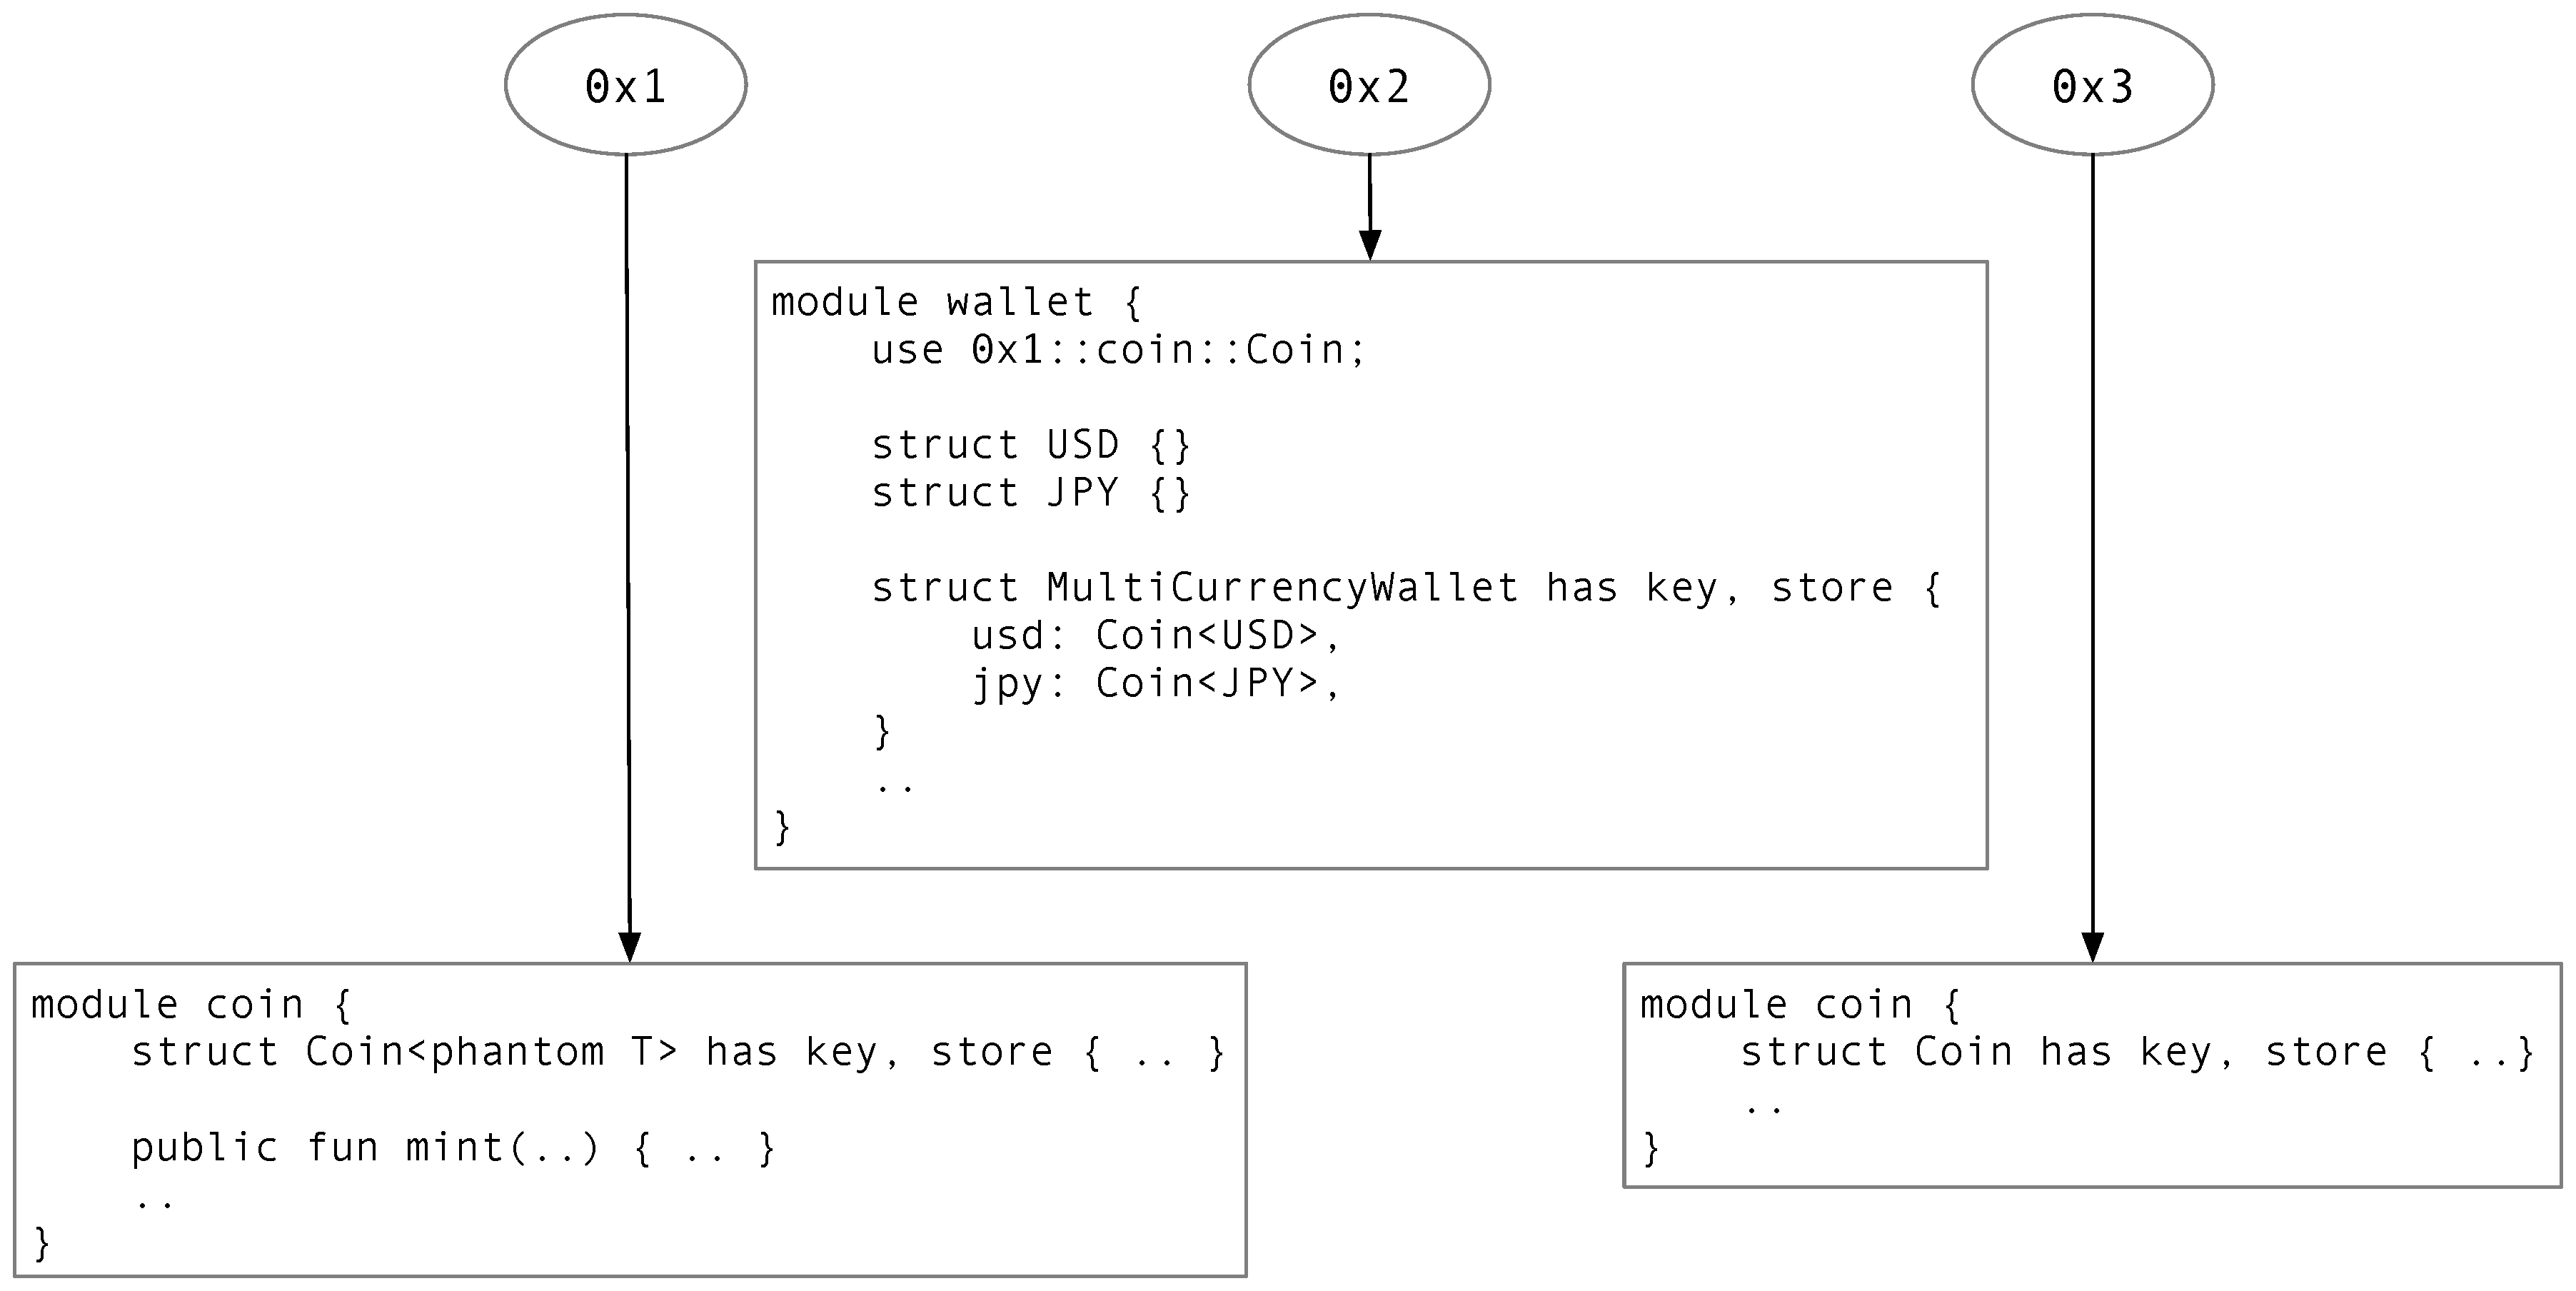
\includegraphics[width=0.85\textwidth]{move_1.eps}
\caption{\label{fig:move_modules}Example on-chain Move modules.}
\end{figure}

\subsection{Move modules}

A Move module contains Move bytecode that declares data types (structs) and procedures. It is identified by the address of the account where the module is declared along with a module name. For example, the identifier for the first currency module in Figure \ref{fig:move_modules} is \mintinline{rust}{0x1::coin}. A module can depend on other on-chain modules, as shown by the wallet module in Figure \ref{fig:move_modules}, enabling code reuse.

A module must be uniquely named within an account, i.e., each account can declare at most one module with any given name. For example, the account at address 0x1 in Figure \ref{fig:move_modules} could not declare another module named \mintinline{rust}{coin}. On the other hand, the account at address \mintinline{rust}{0x3} could declare a module named \mintinline{rust}{coin} and the identifier of this module would be \mintinline{rust}{0x3::coin}. Note that \mintinline{rust}{0x1::coin::Coin} and \mintinline{rust}{0x3::coin::Coin} are distinct types and cannot be used interchangeably nor share common module code. In contrast, \mintinline{rust}{0x1::coin::Coin<0x2::wallet::USD>} and \mintinline{rust}{0x1::coin::Coin<0x2::wallet::JPY>} are different instantiations of the same generic type that cannot be used interchangeably but can share common module code.

Modules are grouped into \emph{packages} located at the same address. An owner of this address publishes the package as a whole on-chain, including the bytecode and package metadata. The package metadata determines whether a package can be upgraded or is immutable. For an upgradeable package, compatibility checks are performed before the upgrade is permitted: no existing entry point functions must be changed and no resources can be stored in memory. However, new functions and resources can be added. 

The Aptos framework, consisting of the core libraries and configuration for the Aptos blockchain, is defined as a regular upgradeable package of modules (see Section \ref{subsec:network_governance}).

\subsection{Resources}
\label{subsec:resources}

Similar to modules, account addresses can also have data values associated with them. Within each account address, the values are keyed by their types, with at most one value of each type belonging to the account. Figure \ref{fig:move_data} provides an example of this. Address 0x50 holds a single value, with \mintinline{rust}{0x3::coin::Coin} being the fully-qualified type. \mintinline{rust}{0x3} is the address where the coin module is stored, \mintinline{rust}{coin} is the name of the module and \mintinline{rust}{Coin} is the name of the data type. Values of generic types are also allowed, with different instantiations being treated as distinct types. This is essential for extensibility, allowing different instantiations to share the same functional code.

The rules for mutating, deleting, and publishing a value are encoded in the module that defines the data type. Move’s safety and verification rules prevent other code or entities from directly creating, modifying, or deleting instances of data types defined in other modules.

\begin{figure}
\centering
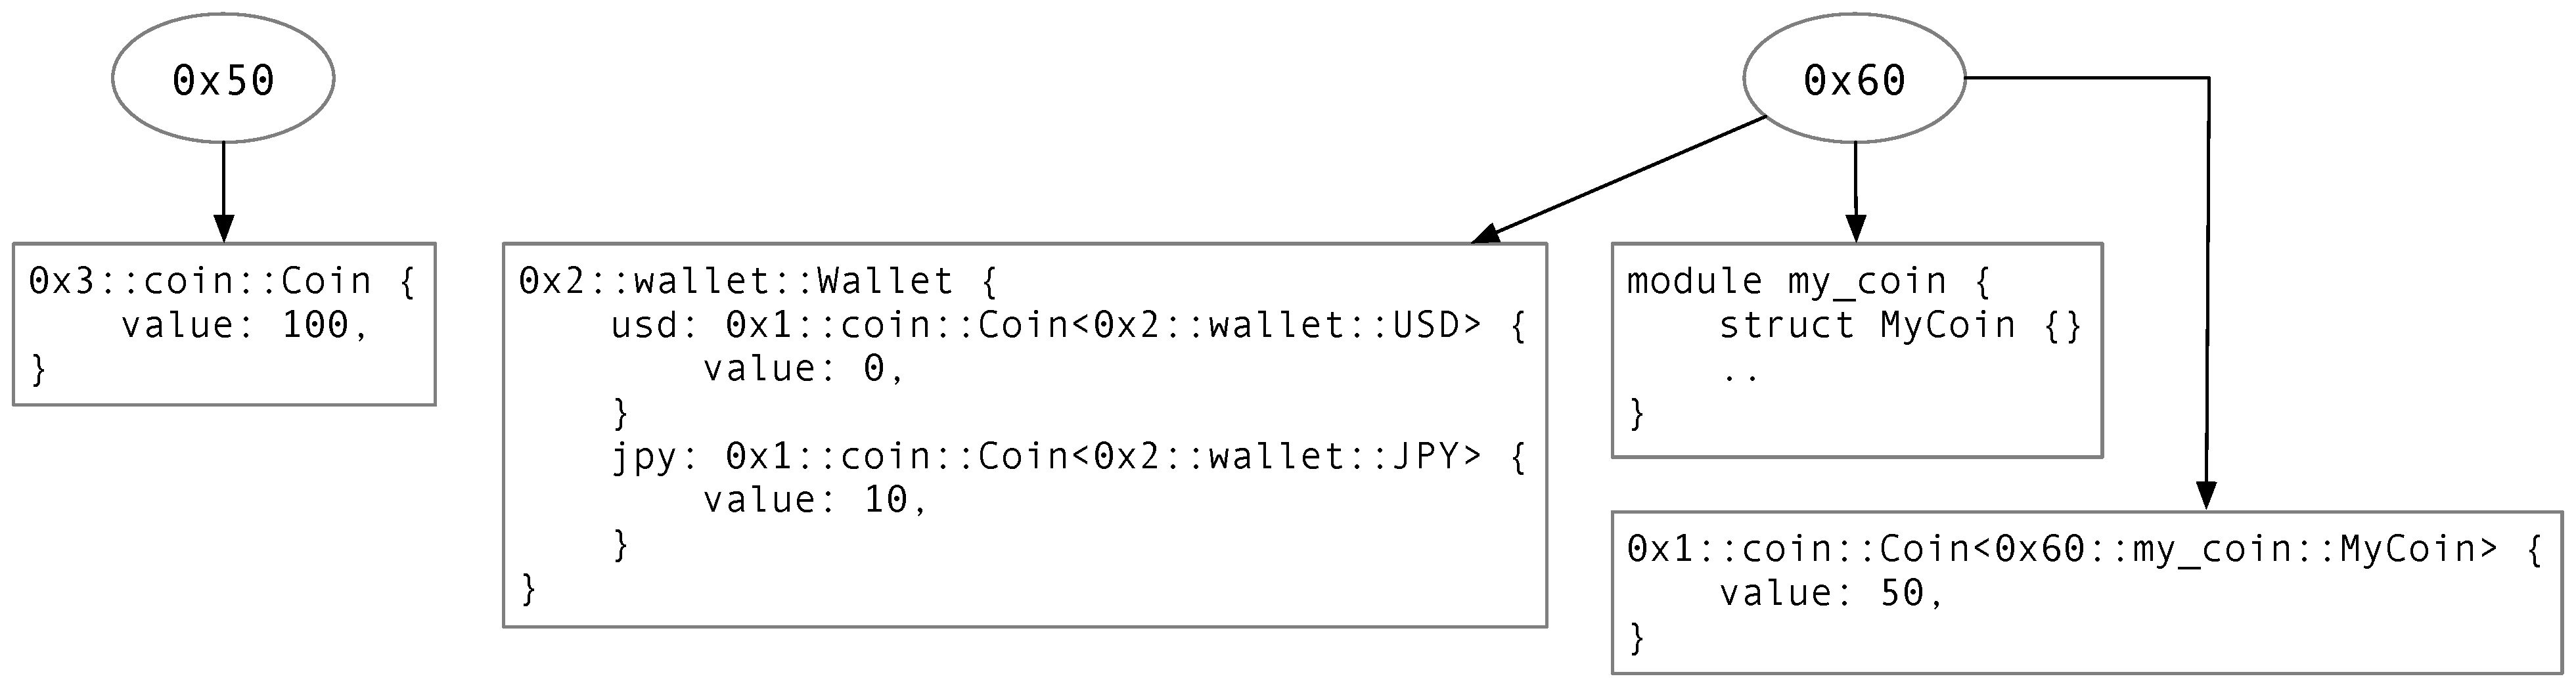
\includegraphics[width=1.0\textwidth]{move_2.eps}
\caption{\label{fig:move_data}Example on-chain data.}
\end{figure}

Having at most one top-level value of each type under an address may at first sound limiting. However, this is not a problem in practice as programmers can define wrapper types with other data as internal fields, thus avoiding any limitations. The \mintinline{rust}{Wallet} struct in Figure \ref{fig:move_data} is an example of how to use wrapper types.

It should also be noted that not all data types can be stored on-chain. For data instances to qualify as top-level values, the data type must have the \mintinline{rust}{key} ability. Similarly, the \mintinline{rust}{store} ability is required for nested values. Data types with both abilities are also called \emph{resources}.

\subsection{Ledger state}
\label{sub:ledger_state}

From the perspective of the Move virtual machine (Move VM), each account consists of a set of values and key-value data structures. These data structures are called \emph{table entries} and are stored in the Binary Canonical Serialization format (BCS). This data layout enables developers to write smart contracts that can operate efficiently on small amounts of data replicated across a large number of accounts, as well as on large amounts of data stored in a small number of accounts. Move modules are stored similarly to account data but under an independent namespace. The genesis ledger state defines the initial set of accounts and their associated state at blockchain initialization.

At launch, the Aptos blockchain will be represented by a single ledger state. However, as adoption increases and technology develops, Aptos will scale up the number of shards to increase throughput (i.e., enable multiple ledger states) and support transactions that move or access assets across shards. Each ledger state will maintain all on-chain assets for the specific shard and provide the same account model with a fine-grained, key-value data store offering near-fixed costs for storage access. 

\section{A safe user experience}
\label{sec:user}

To reach billions of Internet users, the web3 user experience must be safe and accessible. In the sections below, we describe several innovations provided by the Aptos blockchain that work towards this goal.

\subsection{Transaction viability protection}
\label{subsec:transaction_replay_protection}

Signing a transaction means that the signer authorizes the transaction to be committed and executed by the blockchain. Occasionally, users may sign transactions unintentionally or without fully considering all the ways in which their transactions might be manipulated. To reduce this risk, the Aptos blockchain constrains the viability of every transaction and protects the signer from unbounded validity. There are currently three different protections provided by the Aptos blockchain - the sender's sequence number, a transaction expiration time, and a designated chain identifier.
\begin{itemize}
\item A transaction's sequence number can only be committed exactly once for each sender's account. As a result, senders can observe that if the current account sequence number is $\geq$ the sequence number of a transaction $t$, then either $t$ has already been committed or $t$ will never be committed (as the sequence number used by $t$ has already been consumed by another transaction).
\item The blockchain time advances with high precision and frequency (typically sub-second), as detailed in Section \ref{subsubsec:blockchain_time}. If the blockchain time exceeds the expiration time of transaction $t$, then similarly, either $t$ has already been committed or $t$ will never be committed.
\item Every transaction has a designated chain identifier to prevent malicious entities from replaying transactions between different blockchain environments (e.g., across a testnet and mainnet).
\end{itemize}

\subsection{Move-based key management}

As discussed in Section \ref{sec:accounts}, Aptos accounts support key rotation, an important feature that can help reduce the risks associated with private key compromise, long-range attacks, and future advances that might break existing cryptographic algorithms.  In addition, Aptos accounts are also flexible enough to enable new hybrid models of custody. In one such model, a user can delegate the ability to rotate the account's private key to one or more custodians and other trusted entities. A Move module can then define a policy that empowers these trusted entities to rotate the key under specific circumstances. For example, the entities might be represented by a $k$-out-of-$n$ multi-sig key held by many trusted parties and offer key recovery services to prevent user key loss (e.g., 20\% of Bitcoin is currently locked up in unrecoverable accounts \cite{lost_passwords}). 

Moreover, while many wallets support various key recovery schemes, such as backing up private keys to cloud infrastructure, multi-party computation, and social recovery, they are typically implemented without blockchain support (i.e., off-chain). As a result, each wallet needs to implement its own key management infrastructure and related operations become opaque to users. In contrast, supporting key management functionality at the Aptos blockchain layer provides full transparency of all key-related operations and makes it simpler to implement a wallet with rich key management.

\subsection{Pre-signing transaction transparency}

Today, wallets provide very little transparency about the transactions they sign. As a result, users are often easily tricked into signing malicious transactions that may steal funds and have devastating consequences. This is true even for blockchains that require enumerating all on-chain data accessed by each transaction. As a result, there are few user safeguards currently in place, making users vulnerable to a wide variety of attacks. 

To address this, the Aptos ecosystem provides services for \emph{transaction pre-execution}: a precautionary measure that describes to users (in human-readable form) the outcomes of their transactions \emph{prior} to signing. Pairing this with a known history of prior attacks and malicious smart contracts will help to reduce fraud. In addition, Aptos also enables wallets to dictate constraints on transactions during execution. Violating these constraints will result in the transactions being aborted, to further protect users from malicious applications or social engineering attacks.

\subsection{Practical light client protocols}
Relying solely on the TLS/SSL certificates of API providers to establish trust between blockchain clients and servers does not protect clients sufficiently. Even in the presence of valid certificates, wallets and clients have no guarantees as to the authenticity and integrity of the data being presented to them. As a result, API providers may return incorrect or malicious blockchain data, deceiving third parties and performing double-spend attacks.

To prevent this, Aptos provides state proofs and light client verification protocols that can be used by wallets and clients to verify the validity of data being presented by an untrusted third-party server. Moreover, by leveraging the timestamp-based state proofs in Section \ref{subsubsec:period_state_certification}, light clients can always ensure tight bounds on the freshness of account state (e.g., within seconds) and only need to track changes in the network configuration (\emph{epoch changes}) or use current trusted checkpoints (\emph{waypoints}) to stay up-to-date \cite{waypoints}. By combining high-frequency timestamps and inexpensive state proofs, the Aptos blockchain provides increased security guarantees to clients. 

In addition, Aptos nodes also expose rich, high-performance storage interfaces that can be further fine-tuned to allow subscriptions to proofs targeting specific data and accounts on-chain. This can be leveraged by light clients to retain minimal verifiable data without the need to run a full node or process a substantial number of transactions.

\section{Pipelining, batching, and parallel transaction processing}
\label{sec:pipelining_batching}

To maximize throughput, increase concurrency, and reduce engineering complexity, transaction processing on the Aptos blockchain is divided into separate stages. Each stage is completely independent and individually parallelizable, resembling modern, superscalar processor architectures. Not only does this provide significant performance benefits, but also enables the Aptos blockchain to offer new modes of validator-client interaction. For example:
\begin{itemize}
\item Clients can be notified when specific transactions have been included in a batch of persisted transactions. Persisted and valid transactions are highly likely to be committed imminently.
\item Clients can be informed when a batch of persisted transactions has been ordered. Thus, to reduce the latency of determining the executed transaction outputs, clients can select to execute transactions locally rather than wait for the validators to complete execution remotely.
\item Clients can elect to wait for certified transaction execution by the validators and perform state synchronization on the attested results (e.g., see Section \ref{sub:state_sync}).
\end{itemize}
The Aptos modular design aids development speed and supports faster release cycles, as changes can be targeted to individual modules, instead of a single monolithic architecture. Similarly, the modular design also provides a structured path to scaling validators beyond a single machine, providing access to additional compute, network, and storage resources. Figure \ref{fig:pipeline} shows the transaction life cycle across the various processing stages.

\begin{figure}
\centering
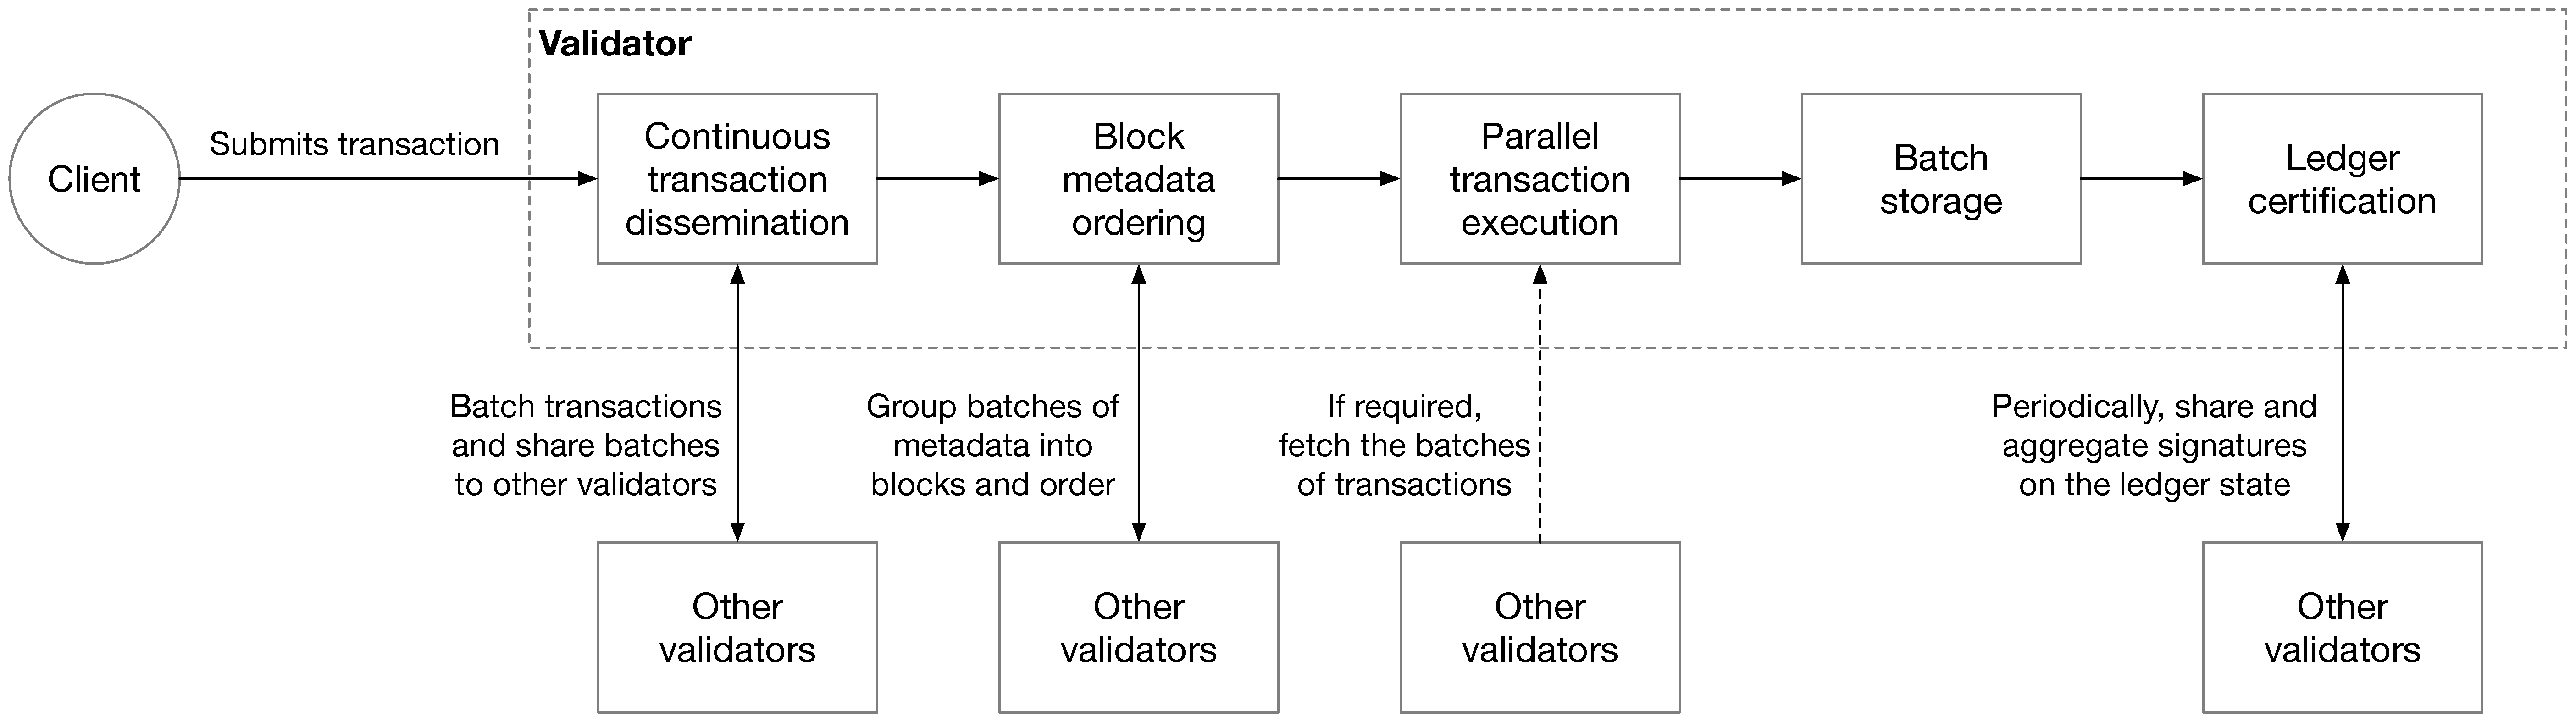
\includegraphics[width=1.0\textwidth]{pipeline.eps}
\caption{\label{fig:pipeline}The transaction processing life cycle. All stages are completely independent and are individually parallelizable.}
\end{figure}

\subsection{Batch processing}

Batch processing is an important efficiency optimization that is part of every phase of operation in the Aptos blockchain. Transactions are grouped into batches by each validator during transaction dissemination, and batches are combined into blocks during consensus. The execution, storage, and ledger certification phases also work in batches to provide opportunities for reordering, reduction of operations (e.g., duplicate computation or signature verification), and parallel execution.

Grouping transactions into batches can induce small amounts of latency, for example, waiting 200 milliseconds to accumulate a batch of transactions before performing dissemination. However, batching is easily configurable with respect to a maximum waiting period and maximum batch size, enabling a decentralized network to automatically optimize across latency and efficiency. Batching also allows for efficient fee markets to prioritize transactions and avoid unintended denial-of-service (DoS) attacks from overzealous clients.

\subsection{Continuous transaction dissemination}
\label{continuous_txn_dissemination}

Following the primary insight of Narwhal \& Tusk \cite{narwhal_tusk}, transaction dissemination in the Aptos blockchain is decoupled from consensus. Validators continuously stream batches of transactions to each other, utilizing all available network resources concurrently. Each batch distributed by a validator $v$ is persisted, and a signature on the batch digest is sent back to $v$. Following the consensus requirements defined in Section \ref{subsec:block_metadata_ordering}, any $2f+1$ stake weighted signatures on the batch digest form a proof of availability (PoAv). Such a proof guarantees that at least $f+1$ stake weighted honest validators have stored the batch, and thus all honest validators will be able to retrieve it prior to execution. 

Infinitely persisting batches of transactions can open a DoS attack vector by causing validators to run out of storage and crash. To prevent this, each batch of transactions has an associated timestamp. The timestamp on the batch allows efficient garbage collection at each validator. In addition, a separate per-validator quota mechanism is designed to protect validators from running out of space even in the most extreme circumstances, such as under potential byzantine attacks. Batches also have sizing constraints that are validated prior to agreement to persist to stable storage. Finally, several optimizations to de-duplicate and cache transactions reduce storage costs and ensure performant integration with the parallel execution engine.

\begin{figure}
\centering
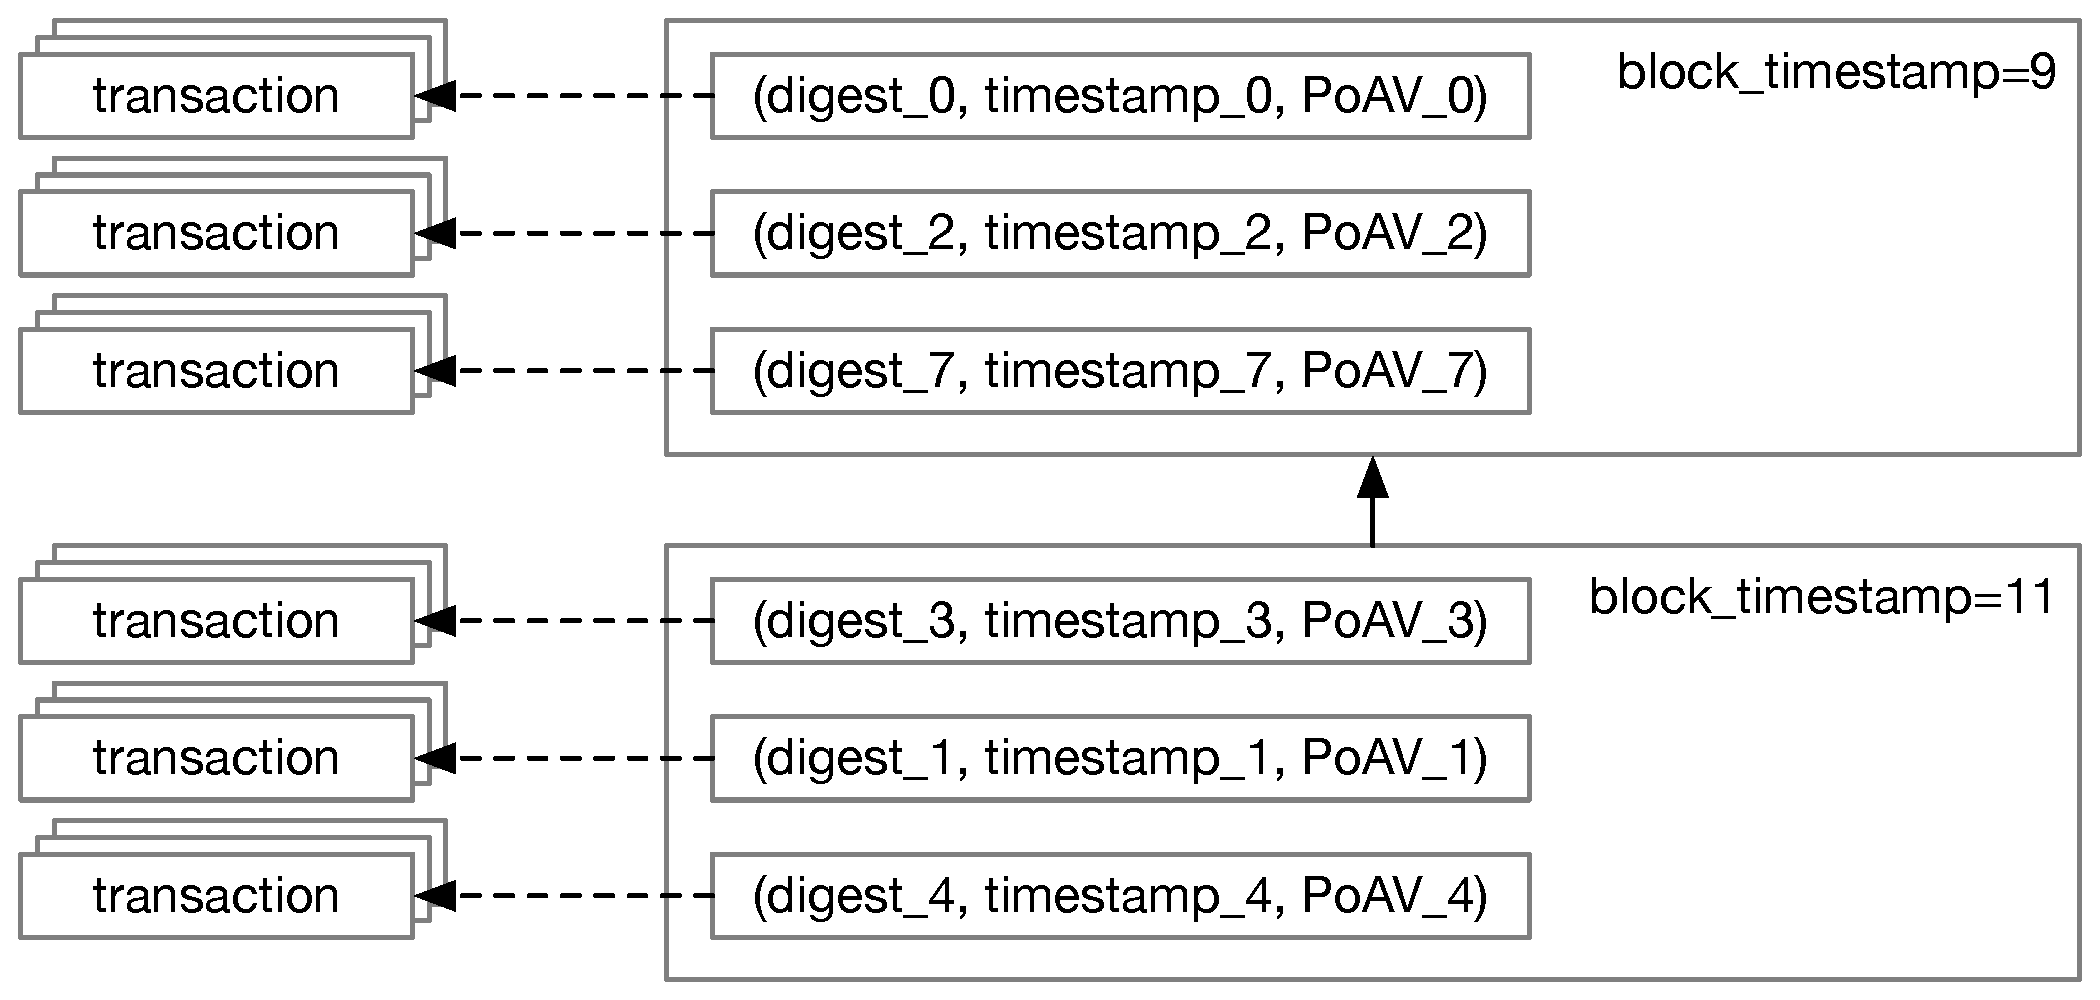
\includegraphics[width=0.8\textwidth]{ordering.eps}
\caption{\label{fig:block}Block metadata ordering occurs independently from transaction dissemination.}
\end{figure}

\subsection{Block metadata ordering}
\label{subsec:block_metadata_ordering}

One common misconception is that consensus is slow and therefore the primary bottleneck for blockchain throughput and latency. One of the key innovations of the Aptos blockchain is to decouple non-agreement related tasks out of the consensus phase, such as transaction dissemination, transaction execution/storage, and ledger certification. By decoupling transaction dissemination from the consensus phase, ordering can occur with very low bandwidth (block metadata and proofs only), resulting in high transaction throughput and minimized latency.

Today, the Aptos blockchain leverages the latest iteration of DiemBFTv4 \cite{diembft_v4}, an optimistically responsive BFT consensus protocol. Consensus in the common case only requires two network round trips (with round trip times typically less than 300 milliseconds worldwide) and dynamically adjusts to faulty validators through a leader reputation mechanism \cite{be_aware}. The on-chain leader reputation mechanism promotes validators that have successfully committed blocks in a window and demotes validators that are not participating. This novel mechanism significantly improves performance in decentralized environments, correspondingly provides infrastructure for appropriate incentives, and quickly minimizes the impact of failed validators on throughput and latency.

DiemBFTv4 guarantees liveness under partial synchrony and ensures safety under asynchrony where the total validator stake is $\geq 3f+1$ with up to $f$ stake-weighted faulty validators. DiemBFTv4 has been extensively tested in several iterations since 2019 with dozens of node operators and a multi-wallet ecosystem. We are also experimenting with our recent research (e.g., Bullshark \cite{bullshark}) and other protocols that rely on the block history and associated communication to determine block metadata ordering and finality.

A consensus block and a proposal timestamp are proposed by a leader and agreed upon by the other validators as shown in Figure \ref{fig:block}. Note that each consensus block contains only the batch metadata and proofs. Actual transactions are not required in the block, as the PoAV ensure that the batches of transactions will be available at the execution phase after ordering (see Section~\ref{continuous_txn_dissemination}). Validators may vote on a leader's proposal after verifying the proof and the block metadata criteria are met (e.g., proposal timestamp $\le$ block expiration time).

\subsubsection{Blockchain time}
\label{subsubsec:blockchain_time}

The Aptos blockchain adopts an approximate, agreed-upon, physical timestamp for every proposed block, and correspondingly, all transactions within that block. This timestamp enables many important use cases. For example:
\begin{itemize}
\item Time-dependent logic in smart contracts. For instance, a developer would like to encode that all bids on an auction must be received prior to noon on Thursday.
\item As oracles publish on-chain data, an accurate and trusted on-chain timestamp is required to correlate events and handle delays from real-world data.
\item Clients can discern how up-to-date they are with respect to the blockchain. For security reasons, to avoid stale data and long-range attacks, a client should have access to a high-precision timestamp on when the account state was updated.
\item Auditing the blockchain with a well-trusted timestamp provides a strong correlation to off-chain events, such as ensuring that legally-enforced payouts meet expected requirements. 
\item Transaction expiration is based on the most recent committed timestamp. As an additional safeguard for client transactions, clients can select an expiration time for a transaction, as described in Section \ref{subsec:transaction_replay_protection}.
\end{itemize}
The Aptos blockchain provides the following guarantees with respect to timestamps for all transactions within a block:
\begin{itemize}
\item Time is monotonically increasing in the blockchain. That is, if block $B1 < $ block $B2$, then $B1.Time < B2.Time$.
\item If a block of transactions is agreed on with timestamp $T$, then at least $f+1$ honest validators have decided that $T$ is in the past. An honest validator will only vote on a block when its own clock $\ge$ timestamp $T$. See Section \ref{continuous_txn_dissemination}.
\item If a block of transactions has a quorum of signatures in consensus with timestamp $T$, an honest validator will not serve such a block to other validators until its own clock $\ge$ timestamp $T$.
\end{itemize}
The most recent timestamp is updated on every committed block and used as the timestamp for all transactions in that block. When the network is synchronous, a block of transactions is committed every single network round trip and provides a fast updating and highly reliable clock.  A finer granularity of ordering within blocks of transactions can be determined if desired.

\subsection{Parallel transaction execution}
\label{subsec:parallel_transaction_execution}

Once consensus block metadata is ordered, transactions can be executed by any validator, full node, or client. At least $2f+1$ stake weighted validators have veritably persisted transactions for the proposed batches. Since transaction dissemination is continuous, additional honest validators will receive the transaction batches over time. If an honest validator has not received the transactions for the ordered batches by the time it reaches the execution stage, it can download them from the $2f+1$ stake weighted validators, knowing that at least $f+1$ stake weighted validators ( $\ge$ half of the stake weighted PoAV signers) are honest.   

An important goal for any blockchain is to enable as much parallel execution as possible.  The Aptos blockchain advances this direction forward from both the data model and the execution engine.

\subsubsection{Parallel data model}

The Move data model natively supports global addressing of data and modules.  Transactions that do not have overlapping conflicts in data and accounts can execute in parallel.  Given the pipelined design used by the Aptos blockchain, reordering a group of transactions can reduce the number of conflicts, thereby improving concurrency.

Even when transactions modify the same set of on-chain values, much of the transaction execution process can still be parallelized. The Aptos blockchain introduces a new concept, \emph{delta writes}, that describes a modification to account state rather than the modified account state (e.g., increment an integer rather than simply determine the final value). All of the transaction processing can be completed in parallel, and then delta writes are applied in the correct sequence for conflicting values to ensure deterministic results.

Over time, the Aptos blockchain will continue to enhance the data model in ways that improve concurrency (e.g., leverage read/write hints) and also improve ergonomics, making it more natural for developers to create, modify, and compose on-chain values. Move provides flexibility to make these improvements at both the language level and also through platform-specific functionality.

\begin{figure}
\centering
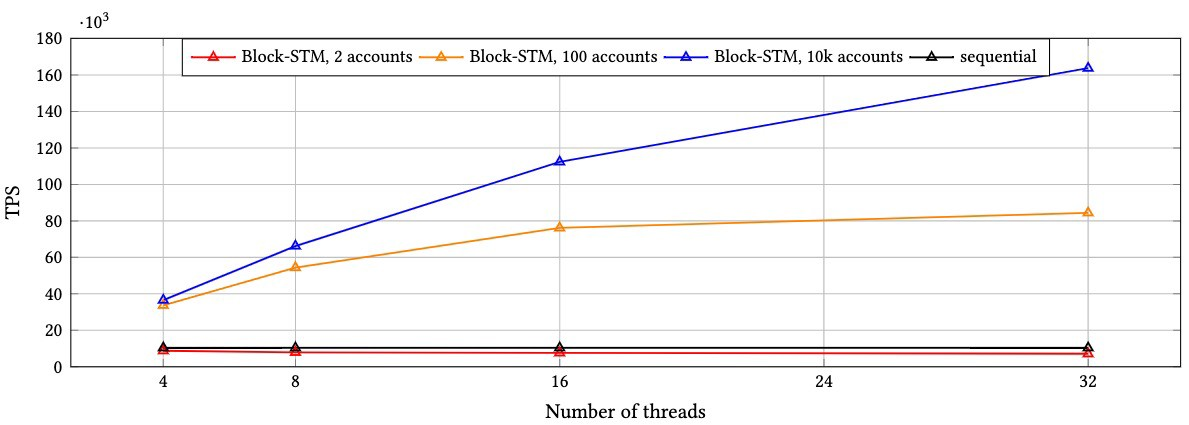
\includegraphics[width=0.95\textwidth]{perf.jpg}
\caption{\label{fig:perf}Block-STM (component-only) benchmarks comparing the number of physical cores with different levels of contention.}
\end{figure}

\subsubsection{Parallel execution engine}

The Block-STM parallel execution engine detects and manages the conflicts for an ordered set of transactions along with optimistic concurrency control to allow for maximum parallelism given a particular ordering \cite{block_stm}.

Batches of transactions are executed optimistically in parallel and validated post-execution. Unsuccessful validations lead to re-executions. Block-STM uses a multi-version data structure to avoid write-write conflicts. All writes to the same location are stored along with their versions, which contain their transaction IDs and the number of times the writing transaction was optimistically re-executed. When transaction $tx$ reads a memory location, it obtains from the multi-version data structure the value written to this location by the highest transaction that appears before $tx$ in the preset order, along with the associated version. 

Block-STM is already integrated into the Aptos blockchain. To understand the full potential of Block-STM performance, we ran experiments with non-trivial peer-to-peer Move transactions (i.e., 8 reads and 5 writes per transaction) as an isolated, execution-only (not end-to-end) benchmark with an in-memory database. In Figure \ref{fig:perf}, we presents our Block-STM execution results. Every block contains 10k transactions and the number of accounts determines the level of conflicts and contention.

Under low contention, Block-STM achieves 16x speedup over sequential execution with 32 threads, while under high contention, Block-STM achieves over 8x speedup. Unique to other parallel execution engines in the blockchain space, Block-STM is able to dynamically and transparently (without any hints from the user) extract the inherent parallelism from any workload.  In comparison to parallel execution environments that require upfront knowledge of data locations to be read or written, Block-STM can support more complex transactions concurrently. This property leads to fewer yet more efficient transactions, decreases cost, and provides lower latency for users. Perhaps most importantly, splitting an atomic transaction into multiple, smaller transactions breaks the all-or-nothing semantics of a single transaction with complex state outcomes. Pairing expressive transaction semantics with parallel execution in Block-STM enables developers to have the best of both worlds.

Note that the block metadata ordering step does not preclude reordering transactions in the parallel execution phase. Transactions can be reordered across one or more blocks to optimize concurrency for parallel execution. The only requirement is that the reordering must be deterministic across all honest validators. Optimizing for parallel execution as well as adding randomization into the reordering can increase the performance and potentially discourage maximal extractable value (MEV) techniques for profitable validator transaction reordering. ``Order-then-reveal'' MEV resistant strategies can also be incorporated into this pipelined design.

Block-STM and transaction reordering are complementary techniques to increase execution parallelism. They can be combined with transaction read/write access hints for additional concurrency.

\subsection{Batch storage}

The parallel execution phase results in write sets for all transactions in a group. These write sets can be stored in memory for maximum execution speed and then used as a cache for the next block or set of blocks to be executed. Any overlapping writes only need to be written to stable storage once. If a validator fails before storing the in-memory write sets, it can simply resume parallel execution from the block metadata ordering phase. Decoupling the batch storage of write sets from the parallel execution step ensures parallel execution can operate efficiently.  In summary, batching write sets reduces the number of storage operations and takes advantage of more efficient, larger I/O operations.

The amount of memory reserved for write set caching can be manually configured per machine and provides a natural back-pressure mechanism. The granularity of the batches can be different from the granularity of parallel execution blocks if desired to tune for specific I/O and memory environments.

\subsection{Ledger certification}

At this point in the pipeline, every individual validator has computed the new state for a committed block of transactions. However, to efficiently support verified light clients and state synchronization, the Aptos blockchain implements ledger certification for the ledger history as well as the ledger state. One key difference for the Aptos blockchain is that ledger certification is not on the critical path of transaction processing and can even be run completely out-of-band if desired.

\subsubsection{Ledger history certification}
\label{subsubsec:ledger_history_certification}

A validator appends the transactions together with their execution output to a global authenticated ledger data structure. Part of the transaction output is the state write set, consisting of the alterations made to the global state accessible by Move. The short authenticator of this data structure is a binding commitment to a ledger history, which includes the newly executed batch of transactions. Similar to transaction execution, the generation of this data structure is deterministic.

Each validator signs the short authenticator to the new version of the resulting database. Validators share their recent set of signed short authenticators with each other, collectively aggregate quorum-signed short authenticators, and also share the recent quorum-signed short authenticators with one another.

Using this collective signature, clients can trust that a database version represents the complete, valid, and irreversible ledger history according to the BFT properties of the protocol. Clients can query any validator (or any third-party replica of the database, such as a full node) to read a database value and verify the result using the authenticator and a proof of the desired data. 

\subsubsection{Periodic state certification}
\label{subsubsec:period_state_certification}

The entirety of the global state accessible by Move can be summarized to a short authenticator at any point in history, similar to a summary of the ledger history. Due to the random access nature of the global state (unlike the ledger history which is append-only), the cost of maintaining this authentication is significant. Nevertheless, when updating the data structure in a large batch, we can compute the update in parallel and also exploit any overlap among the parts that must be updated when each individual state value changes. The Aptos blockchain deliberately only periodically certifies the global state to reduce duplicate shared updates.

During deterministic and configured intervals, the network issues the state checkpoint transactions that include the global state authenticator as part of their output. Such versions are denoted \emph{state checkpoints}. The larger the gap between two checkpoints, the lower the amortized cost of updating the state authenticated data structure per transaction.

With state checkpoints, one can read any state value from them in a trustless way without storing all of the global state. This ability is useful for applications like incremental state syncing, sharded storage across validators, stateless validator nodes, and storage-constrained light clients. 

However, because the state checkpoints are periodic, getting a proof to a specific version of the ledger state requires either additional transaction execution for the missing state alternations or an inclusion proof of them from the authenticated ledger history. 

State checkpoints are tied to the specific transaction versions in the ledger history, hence bound to the timestamp associated with transaction batches mentioned in Section \ref{sec:pipelining_batching}. With the timestamp, a light client can understand the recency of a proven state value. Without a timestamp, a light client proof can only ensure the validity of a previous state that could be far in the past, which provides little assurance of relevance. Also, timestamps for state proofs are necessary for tracking historical access and auditing purposes, such as calculating the average hourly balance of tokens in a token reserve.

State checkpoints can be derived based on a previous state checkpoint and state alternations in the transaction outputs after it. Hence, persisting state checkpoints to stable storage does not need to be on the critical path for transaction processing. Also, beneficial batching effects exist when persisting the state checkpoints as well. Caching the recent state checkpoints (or rather the delta between them) in memory and dumping only the periodic state checkpoints to stable storage can greatly reduce consumption of storage bandwidth. The way checkpoints are chosen to be persisted does not affect the calculation of the authenticated data structure. Hence, this is a per-node choice: node operators can configure the appropriate trade-off between memory capacity and storage bandwidth.

\section{State synchronization}
\label{sub:state_sync}

The Aptos blockchain aims to provide a high throughput, low latency system for all participants in the ecosystem. As a result, the blockchain must offer an efficient state synchronization protocol to disseminate, verify, and persist blockchain data to light clients, full nodes, and validators \cite{evolution_state_sync}. In addition, the synchronization protocol must also be tolerant of resource constraints and heterogeneity within the network, accounting for different users and use cases. For example, it must allow archival full nodes to verify and persist the entire blockchain history and state, while also enabling light clients to efficiently track only a small subset of the Aptos blockchain state.

To achieve this property, the Aptos blockchain leverages the authenticated ledger history and certified state proofs (see Section \ref{subsubsec:ledger_history_certification}) offered by the validators, full nodes, and other replicators to provide a flexible and configurable synchronization protocol. Specifically, participants in the network can select different synchronization strategies to optimize for their use cases and requirements.

For example, in the case of full nodes, Aptos allows multiple synchronization strategies, including the ability to process all transactions since the beginning of time or skip the blockchain history entirely and synchronize only the latest blockchain state using waypoints. In the case of light clients, strategies include synchronizing partial blockchain states, e.g., specific accounts or data values, and enabling verified state reads, e.g., verified account balance fetching. In all cases, Aptos allows participants to configure the amount and age of the data to fetch, process, and retain.   

By adopting a flexible and configurable approach to state synchronization, Aptos can adapt to a variety of client requirements and continue to offer new and more efficient synchronization strategies in the future.

\section{Community ownership}
\label{sec:community_ownership}

The Aptos blockchain will be owned, operated, and governed by a broad and diverse community. A native Aptos token will be used for transaction and network fees, governance voting on protocol upgrades and on-chain/off-chain processes, and securing the blockchain via a proof-of-stake model. A complete description of Aptos token economics will follow in a future publication.

\subsection{Transaction and network fees}
\label{subsec:network_fees}

All Aptos transactions have a gas unit price (specified in Aptos tokens) that allows validators to prioritize the highest value transactions in the network. Moreover, at every stage of the pipelined model, there are multiple opportunities to discard low-value transactions (allowing the blockchain to operate efficiently when at system capacity). Over time, network fees will be deployed to ensure that the costs of using the Aptos blockchain are proportionate to the real-world costs of hardware deployment, maintenance, and node operation. Furthermore, developers will have the opportunity to design applications with different cost trade-offs between compute, storage, and networking.

\subsection{Network governance}
\label{subsec:network_governance}

Every significant feature change and improvement on the Aptos blockchain will go through several phases, including proposal, implementation, testing, and deployment. This structure creates opportunities for relevant parties and stakeholders to provide feedback, share concerns, and offer suggestions. The final phase, deployment, is typically achieved in two steps. First, a software release with the new functionality will be deployed to each node, and second, the functionality will be enabled, e.g., via a feature flag or on-chain configuration variable.

Each software deployment by the node operators must be backward compatible, to ensure the new software is interoperable with the supported releases. The process of deploying a new software version may span multiple days, to account for operators in different time zones and any external issues. Once a sufficient number of nodes have been upgraded, the enablement of the new functionality can be triggered by a synchronization point, such as an agreed-on block height or epoch change. In emergency conditions (e.g., when downtime is unavoidable), the enablement can be through a manual and forced change by the node operators, and in the worst cases, a hard fork in the network.

In comparison to other blockchains, the Aptos blockchain encodes its configuration on-chain. Every validator has the ability to synchronize with the current state of the blockchain and automatically select the correct configuration (e.g., consensus protocol and Aptos framework version) based on the current on-chain values. Upgrades in the Aptos blockchain are seamless and instant due to this functionality.

To provide flexibility and configurability to the enablement process, the Aptos blockchain will support on-chain governance where token holders can vote with respect to their staked token weights. On-chain voting protocols are public, verifiable, and can be instantaneous. On-chain governance can also support the enablement of non-binary outcomes without software deployment. For example, the on-chain leader election protocol parameters can be modified with on-chain governance whereas a pre-known synchronization point would be unable to handle dynamic modifications since all changes would have to be known ahead of time.

On-chain governance can, over time, be deployed across the entire upgrade management process. As an example:
\begin{enumerate}
\item Token holders vote on-chain about transitioning to a new quantum-resistant signature scheme.
\item Developers implement and verify the new signature scheme and create a new software release.
\item Validators upgrade their software to the new release.
\item Token holders vote on-chain to enable the new signature scheme, the on-chain configuration is updated, and the change takes effect.
\end{enumerate}
As an open source project, the Aptos blockchain will depend on strong community feedback and use on-chain governance to manage the appropriate processes. Off-chain upgrade enablement may still be required under certain conditions, but will be minimized over time.

\subsection{Proof-of-stake consensus}

To participate in transaction validation on the Aptos blockchain, validators must have a minimum required amount of staked Aptos tokens. The staked amounts proportionately affect the $2f+1$ stake weighted \emph{PoAv} during transaction dissemination as well as vote weights and leader selection during block metadata ordering.  Validators decide on the split of rewards between themselves and their respective stakers. Stakers can select any number of validators in which to stake their tokens for a pre-agreed reward split. At the end of every epoch, validators and their respective stakers will receive their rewards via the relevant on-chain Move modules.

Any validator operator with sufficient stake can freely join the Aptos blockchain. All parameters, including the minimum stake required, can be set by the on-chain enablement processes described in Section \ref{subsec:network_governance}.

\section{Performance}
\label{sec:performance}

As mentioned in Section \ref{sec:pipelining_batching}, the Aptos blockchain is able to achieve optimal throughput and hardware efficiency via its parallel, batch optimized, and modular transaction processing pipeline. Additional performance initiatives, such as consensus upgrades, delta writes, transaction hints, and critical path caching, will continue to increase throughput and improve efficiency over time.

Today, blockchain throughput is typically measured in transactions per second. However, given the wide range of costs and complexity across transactions and infrastructures, this is an imprecise method to compare systems. Transaction latency is also equally flawed as the starting and ending points of submission to finality are varied across experiments.

In addition, some systems require apriori knowledge of transaction inputs and outputs and force logical transactions to be split into smaller, less complex transactions. Splitting a transaction results in poor user experiences and artificially impacts latency and throughput, without considering what the developer is trying to accomplish. In contrast, the Aptos approach is to enable developers the freedom to build without limits and to measure throughput and latency with respect to real-world use cases rather than synthetic transactions.

The Aptos blockchain will continue to optimize individual validator performance, as well as experiment with scaling techniques that add more validators to the network. Both directions have distinct trade-offs. Any blockchain with parallel execution capabilities can support additional concurrency by requiring more powerful hardware or even structuring each validator as a cluster of individual machines. However, there are practical limits to the number of global validators that is commensurate to the cost and complexity for validator operators. The rise and popularity of serverless databases in cloud services exemplify how few entities can efficiently deploy and maintain these types of complex distributed systems.

\subsection{Homogeneous state sharding}

 Initially, the Aptos blockchain will be launched with a single ledger state. Over time, the Aptos network will take a unique approach to horizontal scalability while still maintaining decentralization. This will occur through multiple sharded ledger states, each offering a homogeneous API and sharding as a first-class concept. The Aptos token will be used for transaction fees, staking, and governance on all shards.
 
 Data may be transferred between shards through a homogeneous bridge. Users and developers can choose their own sharding schemes depending on their needs. For example, developers can propose a new shard or cluster users within existing shards to achieve high intra-shard connections. Moreover, shards may have different system characteristics. One shard might be compute-optimized with SSDs, and another could be optimized for large hard drives with low compute characteristics. By providing hardware flexibility between different shards, developers can leverage the appropriate system characteristics for their applications.
 
 In summary, homogeneous state sharding provides the potential for horizontal throughput scalability, allows developers to program with a single universal state across shards, and enables wallets to easily incorporate sharded data for their users. This provides significant performance benefits as well as the simplicity of a single unified Move smart contracts platform.

\bibliographystyle{IEEEtran}
\small{
\bibliography{bibtex}
}
\end{document}